
%(BEGIN_QUESTION)
% Copyright 2011, Tony R. Kuphaldt, released under the Creative Commons Attribution License (v 1.0)
% This means you may do almost anything with this work of mine, so long as you give me proper credit

This control system measures and regulates the amount of differential pressure across a gas compressor, by opening a {\it recirculation} valve to let high-pressure discharge gas go back to the low-pressure ``suction'' of the compressor.  This control system needs to be very fast-acting, and currently it is anything but that, as revealed by the open-loop trend shown in the upper-right of this illustration:

$$\includegraphics[width=15.5cm]{i00586x01.eps}$$

Identify what type of problem you think you are dealing with here, as the compressor's differential pressure should {\it not} take several seconds to stabilize following a sudden move by the recirculation valve.  Also suggest a next diagnostic test or measurement to take, explaining how the result(s) of that test help further identify the location and/or nature of the fault.

\vskip 20pt \vbox{\hrule \hbox{\strut \vrule{} {\bf Suggestions for Socratic discussion} \vrule} \hrule}

\begin{itemize}
\item{} Based on the evidence presented, how do you know this problem is definitely {\it not} caused by poor PID controller tuning?
\item{} What other methods exist for controlling differential pressure across a large gas compressor, other than using a recirculation valve?
\end{itemize}

\underbar{file i00586}
%(END_QUESTION)





%(BEGIN_ANSWER)

A good step to take next is to figure out whether the problem is on the output side of the control system or on the input side of the control system.  Is the slow pressure trend real, and the control valve not responding as quickly as it should?  Is the pressure actually changing quickly, but the measurement side of the system not accurately reporting it as it should?

Probably the best first-step here is to actually go to the control valve and observe how fast it responds to step-changes from the controller (manual mode).

%(END_ANSWER)





%(BEGIN_NOTES)


%INDEX% Basics, control loop troubleshooting
%INDEX% Process: compressor differential pressure control

%(END_NOTES)

